% ****** Start of file apssamp.tex ******
%
%   This file is part of the APS files in the REVTeX 4.2 distribution.
%   Version 4.2a of REVTeX, December 2014
%
%   Copyright (c) 2014 The American Physical Society.
%
%   See the REVTeX 4 README file for restrictions and more information.
%
% TeX'ing this file requires that you have AMS-LaTeX 2.0 installed
% as well as the rest of the prerequisites for REVTeX 4.2
%
% See the REVTeX 4 README file
% It also requires running BibTeX. The commands are as follows:
%
%  1)  latex apssamp.tex
%  2)  bibtex apssamp
%  3)  latex apssamp.tex
%  4)  latex apssamp.tex
%
\documentclass[%
 preprint,
%superscriptaddress,
%groupedaddress,
%unsortedaddress,
%runinaddress,
%frontmatterverbose, 
%preprint,
%preprintnumbers,
nofootinbib,
%nobibnotes,
%bibnotes,
 amsmath,amssymb,
 aps,
%pra,
%prb,
%rmp,
%prstab,
%prstper,
%floatfix,
]{revtex4-2}

\usepackage{graphicx}% Include figure files
\usepackage{dcolumn}% Align table columns on decimal point
\usepackage{bm}% bold math
\usepackage{fancyhdr}
\usepackage{hyperref}% add hypertext capabilities
%\usepackage[mathlines]{lineno}% Enable numbering of text and display math
%\linenumbers\relax % Commence numbering lines

%\usepackage[showframe,%Uncomment any one of the following lines to test 
%%scale=0.7, marginratio={1:1, 2:3}, ignoreall,% default settings
%%text={7in,10in},centering,
%%margin=1.5in,
%%total={6.5in,8.75in}, top=1.2in, left=0.9in, includefoot,
%%height=10in,a5paper,hmargin={3cm,0.8in},
%]{geometry}

\renewcommand{\headrulewidth}{0pt}
\fancyhead[L]{
%\includegraphics[width=4cm]{/Users/tomluu/Research/talks/fzjTemplate/uniBonn_logo.jpg}
}
\fancyhead[R]{
\includegraphics[width=4cm]{/Users/tomluu/Research/talks/fzjTemplate/fzj_logo.jpg}
}
\pagestyle{plain}

\begin{document}

\preprint{???}

\title{Contracting the $KN$ and $\overline{K}N$ systems}
\author{Thomas Luu}
\affiliation{Institute for Advanced Simulation 4\\
Forschungszentrum J\"ulich, Germany}
\affiliation{Rheinische Friedrich-Williams-Universit\"at Bonn, Germany}

\author{Jangho Kim}
\affiliation{Institute for Advanced Simulation 4\\
Forschungszentrum J\"ulich, Germany}

\date{\today}% It is always \today, today,
             %  but any date may be explicitly specified

\begin{abstract}
We present notes on performing contractions for the $KN$ and $\overline{K}N$ systems.  These notes are a \emph{work in progress!}  
\end{abstract}

%\keywords{Suggested keywords}%Use showkeys class option if keyword
                              %display desired
\maketitle

%\tableofcontents

\thispagestyle{fancy}

\clearpage{}
%\tableofcontents
%\newpage

\section{Preliminaries}
Here are our assumptions:
\begin{itemize}
\item We work in the isospin limit, $m_u=m_d$.
%\item Correlators are `point-to-all', and the spatial points are summed at the sink to project onto specific momenta $\tilde{p}$.
\item The interpolating operator for the kaon is given by $K^+=\bar{s}\gamma_5 u$ (see, e.g. ref.\cite{Gattringer:2010zz}).  $K^0$ is obtained by isospin lowering.
\item The interpolating operator for the anti-kaon is given by $K^-=\bar{u}\gamma_5s$, and the $\overline{K}^0$ is obtained by isospin raising.
\item The interpolating operators for the nucleon are taken from Basak \emph{et al.}\cite{Basak:2005ir}.  This means that the spinor basis is in the `Dirac-Pauli' basis.  This is important to know when coding up these contractions.
\end{itemize}

\section{Strangeness $S=+1$, isospin $I=1$ ($KN$) system}
This system contains no disconnected diagrams.  The three different systems, corresponding to the different isospin projections $I_z$, are
\begin{eqnarray*}
|1,\ 1\rangle&=&|K^+\rangle\ |p\rangle\\
|1,\ 0\rangle&=&\frac{1}{\sqrt{2}}\left(|K^0\rangle\ |p\rangle + |K^+\rangle\ |n\rangle \right)\\
|1,-1\rangle&=&|K^0\rangle\ |n\rangle\ .
\end{eqnarray*}
These systems are all related via an isospin rotation.  Since we are in the isospin limit, we believe these three systems should be degenerate.  But having contractions for each of these channels would be beneficial since it would add statistics to the calculation (as well as provide cross checks).

\subsection{$|K^+\rangle\ |p\rangle$}
The proton interpolating operator is \cite{Basak:2005ir}
\begin{eqnarray*}
\bar{P}_{\mu_1\mu_2\mu_3}(n)&=&\frac{\epsilon_{abc}}{\sqrt{2}}\left[\bar{d}^a_{\mu_2}(n)\bar{u}^b_{\mu_1}(n)-\bar{d}^a_{\mu_1}(n)\bar{u}^b_{\mu_2}(n)\right]\bar{u}^c_{\mu_3}(n)\\
P_{\mu_1\mu_2\mu_3}(n)&=&\frac{\epsilon_{abc}}{\sqrt{2}}u^c_{\mu_3'}(n)\left[u^b_{\mu_1'}(n)d^a_{\mu_2'}(n)-u^b_{\mu_2'}(n)d^a_{\mu_1'}(n)\right]\ ,
\end{eqnarray*}
where $n$ is the lattice position and we use the usual convention that Roman letters correspond to colour indices and Greek letters are spinor indices.
For a spin $\uparrow$ interpolating operator, table VI of ref.\cite{Basak:2005ir} gives $P_{\uparrow}=P_{121}$, for example.  The general correlator is given by 
\begin{displaymath}
C^{\mu_1'\mu_2'\mu_3'}_{\mu_1\mu_2\mu_3}(m',n';m,n)=\langle P_{\mu_1'\mu_2'\mu_3'}(m')K^+(n')\bar{K}^+(n)\bar{P}_{\mu_1\mu_2\mu_3}(m)\rangle\ .
\end{displaymath}
This gives (summation convention applies here)
\begin{multline}
[\gamma_5]_{\alpha'\beta'}\ [\gamma_5]_{\alpha\beta}\ \epsilon_{a'b'c'}\ \epsilon_{abc}\  \frac{1}{2}\times\\
\langle 
u^{c'}_{\mu_3'}(m')\left[u^{b'}_{\mu_1'}(m')d^{a'}_{\mu_2'}(m')-u^{b'}_{\mu_2'}(m')d^{a'}_{\mu_1'}(m')\right]
\bar{s}_{\alpha'}^i(n')u_{\beta'}^i(n')\\
\bar{u}_{\alpha}^j(n)s_{\beta}^j(n)
\left[\bar{d}^a_{\mu_2}(m)\bar{u}^b_{\mu_1}(m)-\bar{d}^a_{\mu_1}(m)\bar{u}^b_{\mu_2}(m)\right]\bar{u}^c_{\mu_3}(m)\rangle\ .
\end{multline}
These contractions can be split generally into a `direct' and `exchange' part,
\begin{equation}
C^{\mu_1'\mu_2'\mu_3'}_{\mu_1\mu_2\mu_3}(m',n';m,n)=
C^{\mu_1'\mu_2'\mu_3'}_{\mu_1\mu_2\mu_3}(m',n';m,n)_{direct} +
C^{\mu_1'\mu_2'\mu_3'}_{\mu_1\mu_2\mu_3}(m',n';m,n)_{exchange}\ .
\end{equation}
The simplest set of contractions come from the `direct' part, where the up quarks in the kaon interpolating operators are contracted with each other.  This means that no up quarks in the nucleon are contracted with the kaon.  In this case, the contractions represent the direct product of the single kaon and single nucleon correlators,
\begin{equation}
C^{\mu_1'\mu_2'\mu_3'}_{\mu_1\mu_2\mu_3}(m',n';m,n)_{direct}=C(n';n)_{kaon}\ \times\ C^{\mu_1'\mu_2'\mu_3'}_{\mu_1\mu_2\mu_3}(m';m)_{proton}\ .
\end{equation}
The easy part is the kaon correlator,
\begin{eqnarray}
C(n';n)_{kaon} &=& [\gamma_5]_{\alpha'\beta'}\ [\gamma_5]_{\alpha\beta}
\ \langle \bar{s}_{\alpha'}^i(n')u_{\beta'}^i(n') \bar{u}_{\alpha}^j(n)s_{\beta}^j(n)\rangle\\
&=&-[\gamma_5]_{\alpha'\beta'}\ [\gamma_5]_{\alpha\beta}
\ \langle s_{\beta}^j(n)\bar{s}_{\alpha'}^i(n')\rangle \langle u_{\beta'}^i(n') \bar{u}_{\alpha}^j(n)\rangle\ \\
&=&-\mbox{tr}\left[\gamma_5\ S^{-1}(n;n')\gamma_5\ U^{-1}(n';n)\right]\\
&=&-[S^{-1}(n';n)]_{\alpha,\beta}^{i,j\ *}\ [U^{-1}(n';n)]_{\alpha,\beta}^{i,j} \ ,
\end{eqnarray}
where $S^{-1}$ and $U^{-1}$ are the strange and light quark propagators, respectively, and the trace is taken over both spinor and colour space.  In the last line we used the $\gamma_5$-hermiticity to relate the backward propagator to the hermitian complex of the forward propagator (and do not forget that repeated indices are summed in the last line!) .

Now on to the proton correlator.  A basic component of this correlator is
\begin{multline}
p^{\mu_1'\mu_2'\mu_3'}_{\mu_1\mu_2\mu_3}(m';m) = \epsilon_{a'b'c'}\ \epsilon_{abc}\  \frac{1}{2}
\langle u^{c'}_{\mu_3'}(m')\ u^{b'}_{\mu_1'}(m')d^{a'}_{\mu_2'}(m')\ \bar{d}^a_{\mu_2}(m)\bar{u}^b_{\mu_1}(m)\ \bar{u}^c_{\mu_3}(m)\rangle\\
=\frac{ \epsilon_{a'b'c'}\ \epsilon_{abc}}{2}[D^{-1}(m';m)]_{\mu_2',\mu_2}^{a',a}
\langle u^{c'}_{\mu_3'}(m')\ u^{b'}_{\mu_1'}(m')\bar{u}^b_{\mu_1}(m)\ \bar{u}^c_{\mu_3}(m)\rangle\\
=\frac{ \epsilon_{a'b'c'}\ \epsilon_{abc}}{2}[D^{-1}(m';m)]_{\mu_2',\mu_2}^{a',a}
([U^{-1}(m';m)]_{\mu_1',\mu_1}^{b',b}[U^{-1}(m';m)]_{\mu_3',\mu_3}^{c',c}\\
-[U^{-1}(m';m)]_{\mu_1',\mu_3}^{b',c}[U^{-1}(m';m)]_{\mu_3',\mu_1}^{c',b})
\end{multline}
where $D^{-1}$ is also the light quark propagator, but written this way to distinguish flavour.  With this structure, the entire proton correlator is
\begin{multline}
C^{\mu_1'\mu_2'\mu_3'}_{\mu_1\mu_2\mu_3}(m';m)_{proton}=\\
p^{\mu_1'\mu_2'\mu_3'}_{\mu_1\mu_2\mu_3}(m';m) + 
p^{\mu_2'\mu_1'\mu_3'}_{\mu_2\mu_1\mu_3}(m';m) -
p^{\mu_1'\mu_2'\mu_3'}_{\mu_2\mu_1\mu_3}(m';m)  -
p^{\mu_2'\mu_1'\mu_3'}_{\mu_1\mu_2\mu_3}(m';m) \ . 
\end{multline}

For the `exchange' diagrams, after contracting the strange and down quarks, a basic component looks like
\begin{multline}
e^{\mu_1'\mu_2'\mu_3'}_{\mu_1\mu_2\mu_3}(m',n';m,n)=\\
-[\gamma_5]_{\alpha\beta}[S^{-1}(n;n')]_{\beta,\alpha'}^{j,i}[\gamma_5]_{\alpha'\beta'}\frac{ \epsilon_{a'b'c'}\ \epsilon_{abc}}{2}\ [D^{-1}(m';m)]_{\mu_2',\mu_2}^{a',a}\times\\
\langle 
u^{c'}_{\mu_3'}(m')u^{b'}_{\mu_1'}(m')
u_{\beta'}^i(n')
\bar{u}_{\alpha}^j(n)
\bar{u}^b_{\mu_1}(m)\bar{u}^c_{\mu_3}(m)\rangle\ .
\end{multline}
To ensure that this is an `exchange' diagram, one of the up quarks of the kaon needs to be contracted with one of the up quarks in the proton.  Here is an intermediate state in the calculation that ensures this `exchange':
\begin{multline}
e^{\mu_1'\mu_2'\mu_3'}_{\mu_1\mu_2\mu_3}(m',n';m,n)=\\
-[\gamma_5]_{\alpha\beta}[S^{-1}(n;n')]_{\beta,\alpha'}^{j,i}[\gamma_5]_{\alpha'\beta'}\frac{ \epsilon_{a'b'c'}\ \epsilon_{abc}}{2}\ [D^{-1}(m';m)]_{\mu_2',\mu_2}^{a',a}\times\\
\{[U^{-1}(m';n)]_{\mu_3',\alpha}^{c',j} \langle u^{b'}_{\mu_1'}(m')u_{\beta'}^i(n')
\bar{u}^b_{\mu_1}(m)\bar{u}^c_{\mu_3}(m)\rangle\\
-[U^{-1}(m';n)]_{\mu_1',\alpha}^{b',j}\langle u^{c'}_{\mu_3'}(m')u_{\beta'}^i(n')\bar{u}^b_{\mu_1}(m)\bar{u}^c_{\mu_3}(m)\rangle\}\ .
\end{multline}
Finishing the remaining contractions (and applying $\gamma_5$-hermiticity) gives
\begin{multline}
e^{\mu_1'\mu_2'\mu_3'}_{\mu_1\mu_2\mu_3}(m',n';m,n)=\\
-[S^{-1}(n';n)]_{\beta',\alpha}^{i,j\ *}\frac{ \epsilon_{a'b'c'}\ \epsilon_{abc}}{2}\ [D^{-1}(m';m)]_{\mu_2',\mu_2}^{a',a}\times\\
\{[U^{-1}(m';n)]_{\mu_3',\alpha}^{c',j} ([U^{-1}(n';m)]_{\beta',\mu_1}^{i,b} [U^{-1}(m';m)]_{\mu_1',\mu_3}^{b',c} -
[U^{-1}(m';m)]_{\mu_1',\mu_1}^{b',b} [U^{-1}(n';m)]_{\beta',\mu_3}^{i,c} )\\
-[U^{-1}(m';n)]_{\mu_1',\alpha}^{b',j}
([U^{-1}(n';m)]_{\beta',\mu_1}^{i,b} [U^{-1}(m';m)]_{\mu_3',\mu_3}^{c',c} -
[U^{-1}(m';m)]_{\mu_3',\mu_1}^{c',b} [U^{-1}(n';m)]_{\beta',\mu_3}^{i,c} )\}\ .
\end{multline}
With this structure the entire exchange part can be written as
\begin{multline}
C^{\mu_1'\mu_2'\mu_3'}_{\mu_1\mu_2\mu_3}(m',n';m,n)_{exchange}=\\
e^{\mu_1'\mu_2'\mu_3'}_{\mu_1\mu_2\mu_3}(m',n';m,n)+e^{\mu_2'\mu_1'\mu_3'}_{\mu_2\mu_1\mu_3}(m',n';m,n)-
e^{\mu_1'\mu_2'\mu_3'}_{\mu_2\mu_1\mu_3}(m',n';m,n)-e^{\mu_2'\mu_1'\mu_3'}_{\mu_1\mu_2\mu_3}(m',n';m,n)
\end{multline}

\subsubsection{Momentum projection}
Propagators are calculated as `point-to-all' due to computational restrictions.  Further, they are summed over all lattices spatial positions at the sink so as to project on to definite momentum.  The details of this sum are not necessary for these notes (see ref.\cite{Gattringer:2010zz}, for example).  The end result is that propagators have a dependence on source position and sink momentum, for example, $S^{-1}(\tilde{p},n)$.  If one places the kaon interpolating operator at source $n$ and proton interpolating operator at $m$, and require that the kaon at the sink have momentum $\tilde{p}$, and similarly the proton at the sink having $\tilde{q}$, then by looking at the various propagators above (and making the substitutions $m'\rightarrow \tilde{q}, n'\rightarrow\tilde{p}$) we see that we need the following types of quark propagators,
\begin{eqnarray*}
&&S^{-1}(\tilde{p};n)\\
&&U^{-1}(\tilde{p};n)\\
&&U^{-1}(\tilde{p};m)\\
&&U^{-1}(\tilde{q};m)\quad\quad \left(=D^{-1}(\tilde{q};m)\right)\\
&&U^{-1}(\tilde{q};n)\ .
\end{eqnarray*}
So in the isospin limit, using general source locations and momentum projections for both kaon and proton interpolating operators, we see that we need at least 5 different propagator calculations to do this contraction.

\subsubsection{Setting $n=m$ and $\tilde{p}=\tilde{q}=0$}
The simplest scenario in LQCD calculations, and one that is most used (as long as Pauli exclusion principle allows it!), is to to set all the sources at the same point, $m=n$.  Without loss of generality, we label this source position as $0$.  Further, one projects all interpolators at the sink to zero momentum, $\tilde{q}=\tilde{p}=0$.  This simplifies the calculation of this system greatly, since now only two propagators are needed (instead of 5), one for each light and heavy quark.  

\subsection{$\frac{1}{\sqrt{2}}\left(|K^0\rangle\ |p\rangle + |K^+\rangle\ |n\rangle \right)$}
\subsection{$|K^0\rangle\ |n\rangle$}
\section{Strangeness $S=+1$, isospin $I=0$ ($KN$) system}
Here also there are no disconnected diagrams and there is only one system:
\begin{displaymath}
|0,\ 0\rangle=\frac{1}{\sqrt{2}}\left(|K^0\rangle\ |p\rangle - |K^+\rangle\ |n\rangle\right)\ .
\end{displaymath}



\section{Strangeness $S=-1$, isospin $I=1$ ($\overline{K}N$) system}
This system \emph{contains} disconnected diagrams.  The three different isospin projections $I_z$ are
\begin{eqnarray*}
|1,\ 1\rangle&=&|\overline{K}^0\rangle\ |p\rangle\\
|1,\ 0\rangle&=&\frac{1}{\sqrt{2}}\left(|K^-\rangle\ |p\rangle + |\overline{K}^0\rangle\ |n\rangle \right)\\
|1,-1\rangle&=&|K^-\rangle\ |n\rangle\ .
\end{eqnarray*}

\section{Strangeness $S=-1$, isospin $I=0$ ($\overline{K}N$) system}
The relevant state is
\begin{displaymath}
|0,0\rangle=\frac{1}{\sqrt{2}}\left(\left|K^{-}\right\rangle|p\rangle-\left|\bar{K}^{0}\right\rangle|n\rangle\right)
\end{displaymath}
This state has the same quantum numbers as the $\Lambda(1405)$.  The contraction becomes
{\footnotesize
\begin{multline}
\frac{1}{2}\left(\langle P_{\mu_1'\mu_2'\mu_3'}(m')K^-(n')\overline{K}^-(n)\overline{P}_{\mu_1\mu_2\mu_3}(m)\rangle
+
\langle N_{\mu_1'\mu_2'\mu_3'}(m')\overline{K}^0(n')K^0(n)\overline{N}_{\mu_1\mu_2\mu_3}(m)\rangle
\right.\\
-\left.
\langle N_{\mu_1'\mu_2'\mu_3'}(m')\overline{K}^0(n')\overline{K}^-(n)\overline{P}_{\mu_1\mu_2\mu_3}(m)\rangle
-
\langle P_{\mu_1'\mu_2'\mu_3'}(m')K^-(n')K^0(n)\overline{N}_{\mu_1\mu_2\mu_3}(m)\rangle
\right)\\
\equiv
\frac{1}{2}\left(
T^{\mu_1'\mu_2'\mu_3'}_{\mu_1\mu_2\mu_3}(m',n';m,n)
+ U^{\mu_1'\mu_2'\mu_3'}_{\mu_1\mu_2\mu_3}(m',n';m,n)
+ V^{\mu_1'\mu_2'\mu_3'}_{\mu_1\mu_2\mu_3}(m',n';m,n)
+ X^{\mu_1'\mu_2'\mu_3'}_{\mu_1\mu_2\mu_3}(m',n';m,n)
\right)\\
=\left(T^{\mu_1'\mu_2'\mu_3'}_{\mu_1\mu_2\mu_3}(m',n';m,n)+V^{\mu_1'\mu_2'\mu_3'}_{\mu_1\mu_2\mu_3}(m',n';m,n)\right)
\end{multline}
}In the last line we used the fact that we are working in the isospin limit.  We consider each term in turn.

\subsection{$T^{\mu_1'\mu_2'\mu_3'}_{\mu_1\mu_2\mu_3}(m',n';m,n)$ term}
There is a `direct' term and an `exchange' term in this case.  Diagrammatically the `direct' term is shown in \autoref{fig:T_direct}.
\begin{figure}
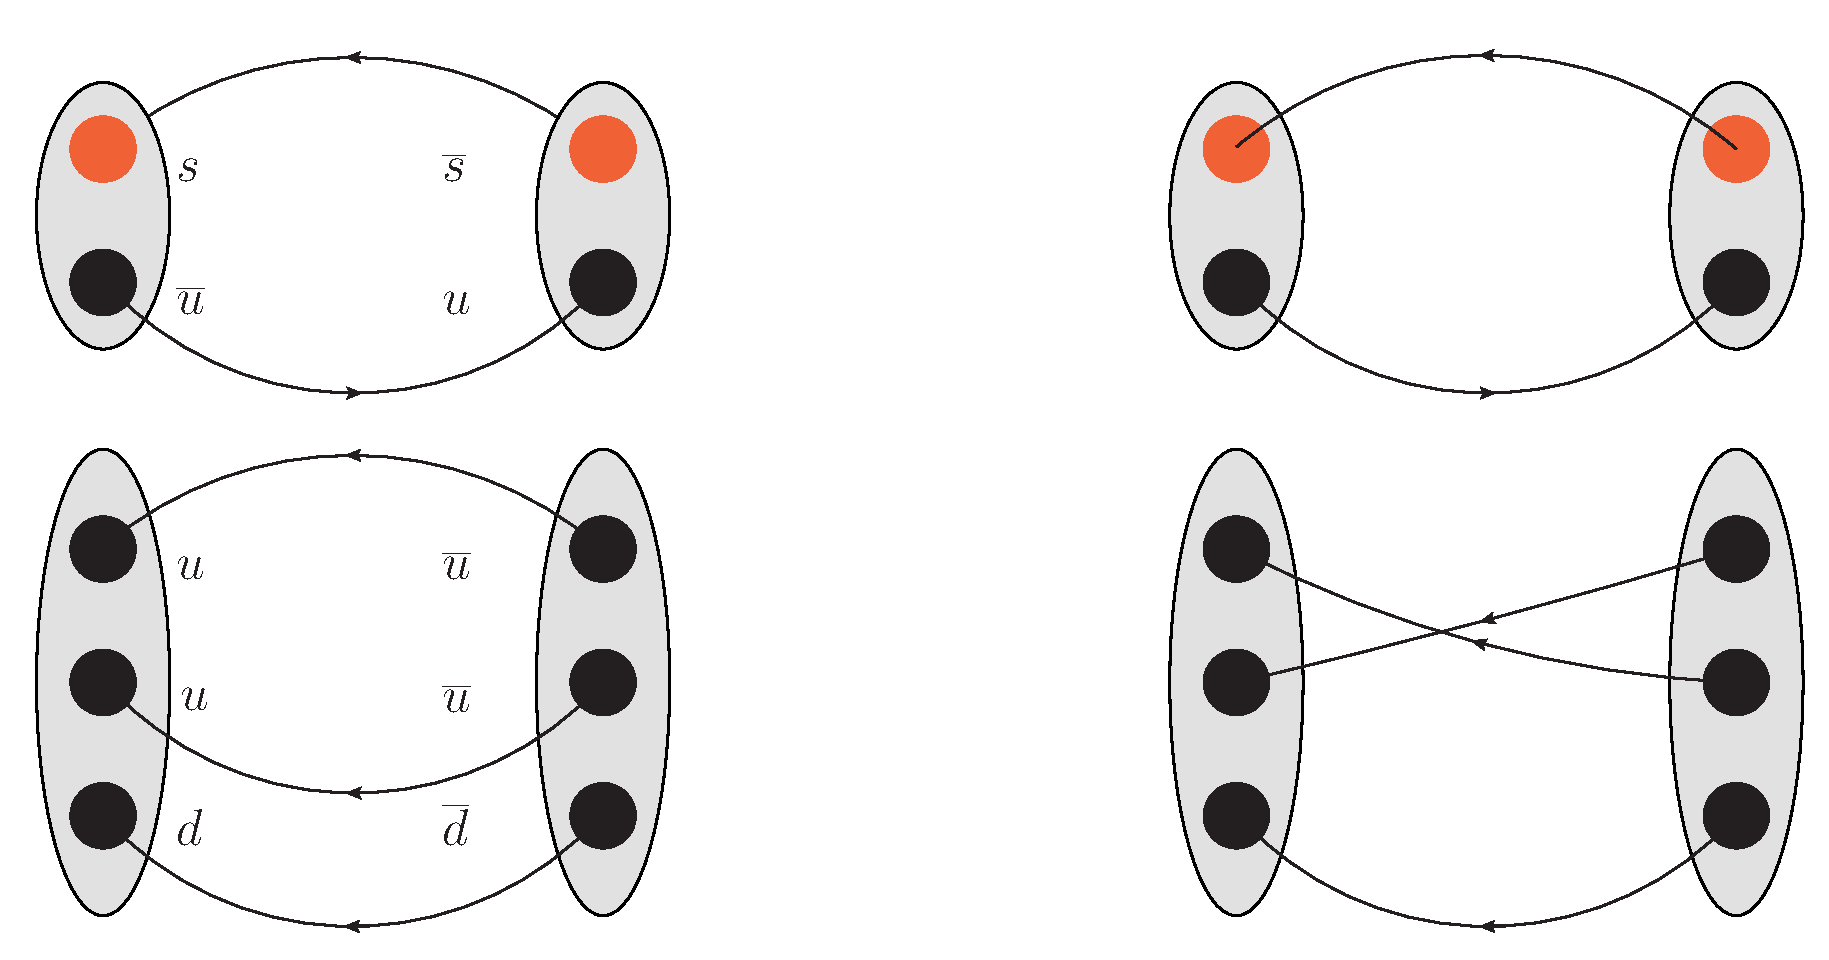
\includegraphics[width=.6\textwidth]{T_direct.eps}
\caption{Direct terms of $T^{\mu_1'\mu_2'\mu_3'}_{\mu_1\mu_2\mu_3}(m',n';m,n)$. \label{fig:T_direct}}
\end{figure}
\begin{figure}
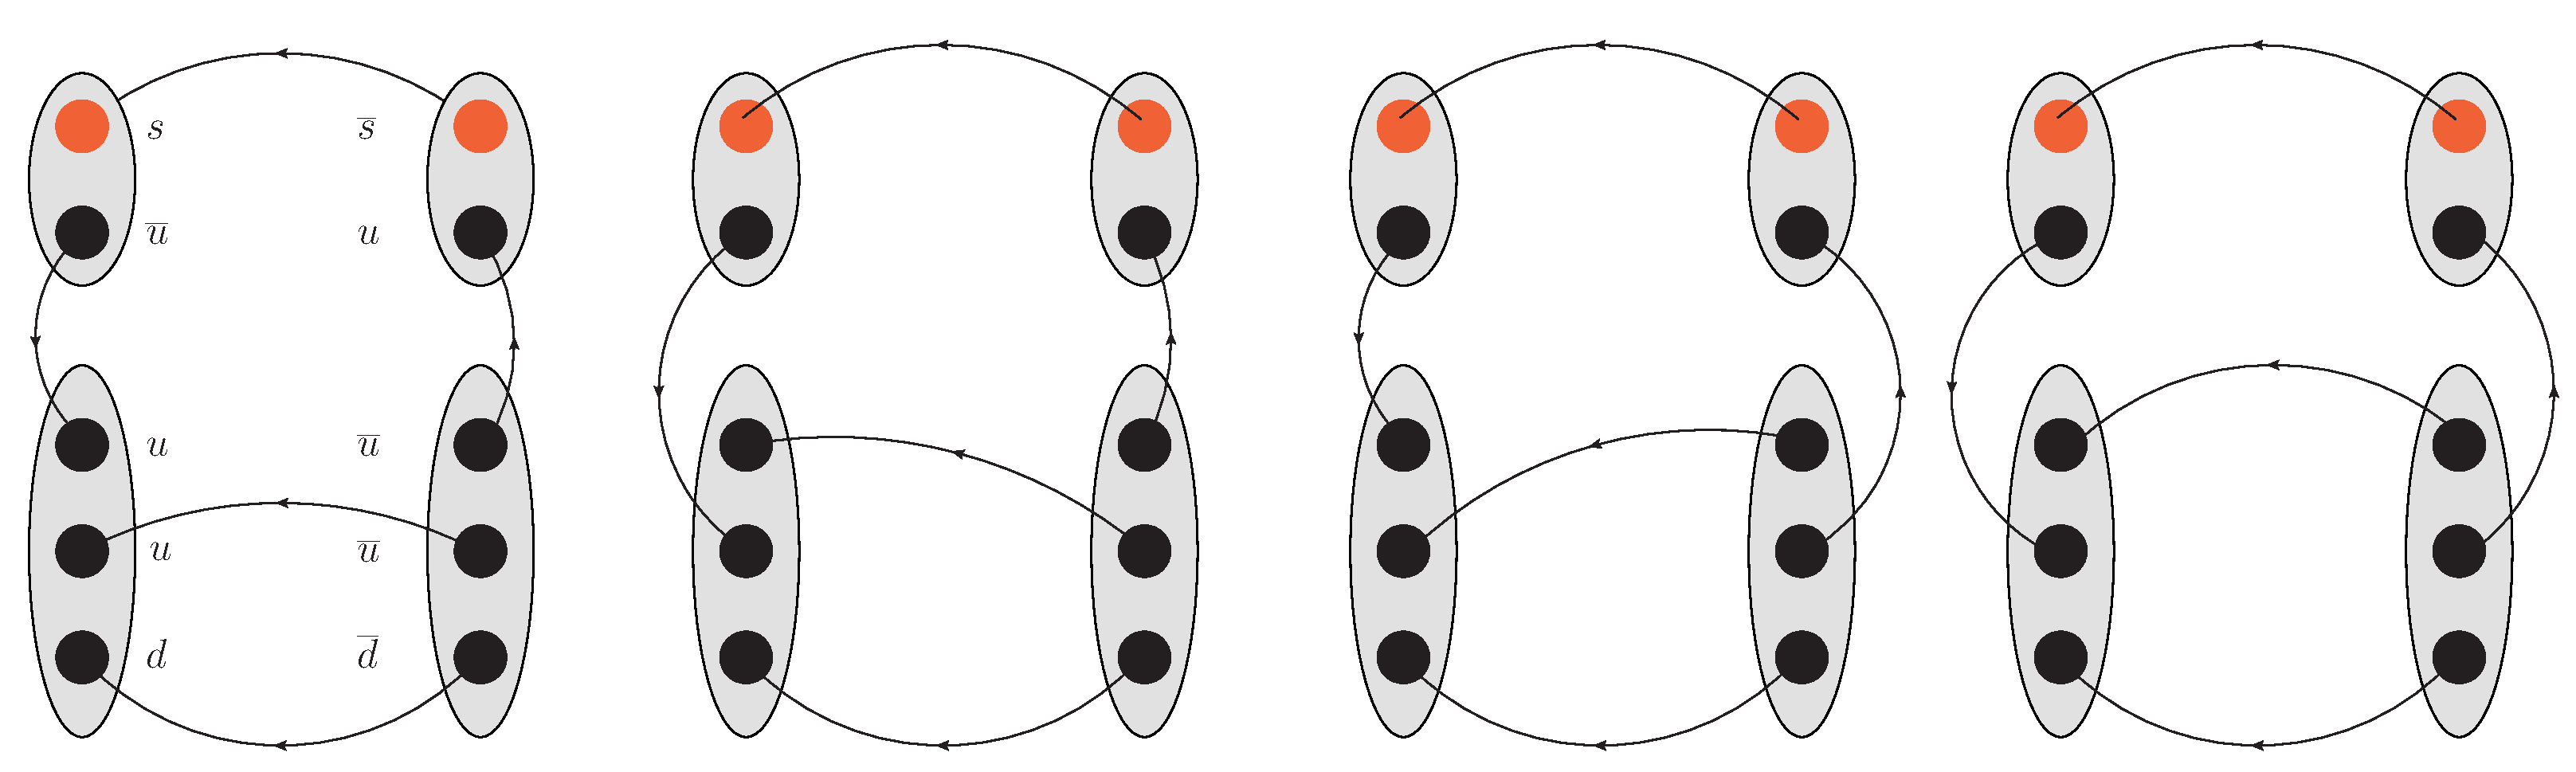
\includegraphics[width=\textwidth]{T_exchange.eps}
\caption{Exchange terms of $T^{\mu_1'\mu_2'\mu_3'}_{\mu_1\mu_2\mu_3}(m',n';m,n)$.  These involve disconnected diagrams. \label{fig:T_exchange}}
\end{figure}
The `exchange' term is shown in \autoref{fig:T_exchange}.  Note that this term has the `single-disconnected' diagrams that will require sequential solves on each timeslice.

\subsection{$U^{\mu_1'\mu_2'\mu_3'}_{\mu_1\mu_2\mu_3}(m',n';m,n)$ term}
In the isospin limit (as well as at the SU3 point), this term is identical to $T^{\mu_1'\mu_2'\mu_3'}_{\mu_1\mu_2\mu_3}(m',n';m,n)$, and therefore diagrammatically this is the same as in \autoref{fig:T_direct} and \autoref{fig:T_exchange}.

\subsection{$V^{\mu_1'\mu_2'\mu_3'}_{\mu_1\mu_2\mu_3}(m',n';m,n)$ term}
This term only has `exchange' type contractions, as shown in \autoref{fig:V_exchange}.  And of course, the are `singly-disconnected'.
\begin{figure}
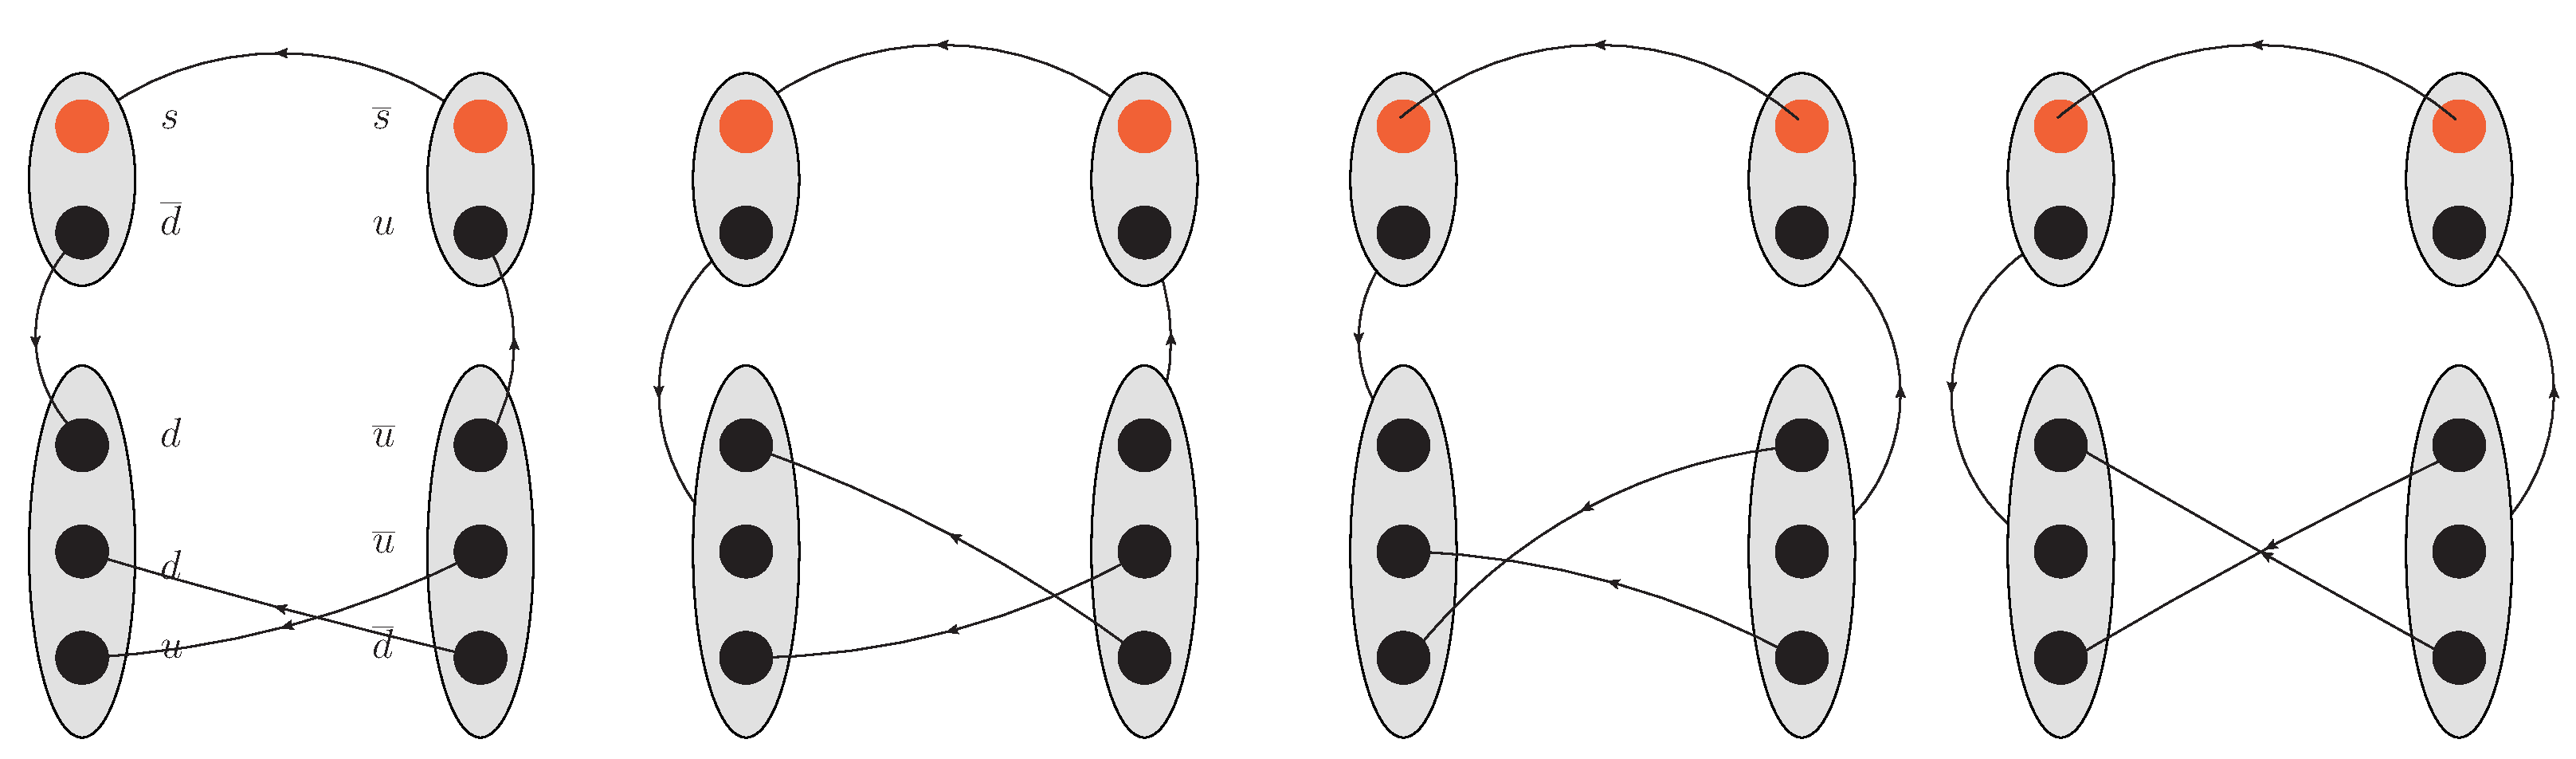
\includegraphics[width=\textwidth]{V_exchange.eps}
\caption{Exchange terms in $V^{\mu_1'\mu_2'\mu_3'}_{\mu_1\mu_2\mu_3}(m',n';m,n)$. \label{fig:V_exchange}}
\end{figure}

\subsection{$X^{\mu_1'\mu_2'\mu_3'}_{\mu_1\mu_2\mu_3}(m',n';m,n)$ term}
Again, isospin limit (and SU3 point) means that this term is identical to $V^{\mu_1'\mu_2'\mu_3'}_{\mu_1\mu_2\mu_3}(m',n';m,n)$.


\section{Connection between SU(3) states and isospin-flavor states}
According to \cite{Roca:2008kr}\footnote{Note the typo in the eq.(9) of the archive version of this paper.  The bottom right matrix element should be $\frac{\sqrt{3}}{2\sqrt{5}}$.}, the transformation between SU(3) states to isospin-flavor states for $S=-1$ and $I=0$ is 
\begin{equation}
\begin{pmatrix}
|\overline{K}N\rangle\\
|\pi\Sigma\rangle\\
|\eta\Lambda\rangle\\
|K\Xi\rangle
\end{pmatrix}
=
\begin{pmatrix}
-\frac{1}{2} & -\frac{1}{\sqrt{10}} & \frac{1}{\sqrt{2}} & -\frac{1}{2} \sqrt{\frac{3}{5}} \\
\frac{1}{2} \sqrt{\frac{3}{2}} & -\sqrt{\frac{3}{5}} & 0 & -\frac{1}{2 \sqrt{10}} \\
-\frac{1}{2 \sqrt{2}} & -\frac{1}{\sqrt{5}} & 0 & \frac{3}{2} \sqrt{\frac{3}{10}} \\
\frac{1}{2} & \frac{1}{\sqrt{10}} & \frac{1}{\sqrt{2}} & \frac{\sqrt{3}}{2 \sqrt{5}}
\end{pmatrix}
\begin{pmatrix}
|{\bf1}\rangle\\
|{\bf8}\rangle\\
|{\bf8'}\rangle\\
|{\bf27}\rangle
\end{pmatrix}
\end{equation}
If we invert this expression we can obtain the singlet and octet representations,
\begin{align}
|{\bf1}\rangle=&-\frac{1 }{2 \sqrt{2}}|\eta \Lambda\rangle-\frac{1}{2}|\overline{K}N\rangle+\frac{1}{2}|K\Xi\rangle+\frac{1}{2} \sqrt{\frac{3}{2}}|\pi \Sigma\rangle\\
|{\bf8}\rangle=&-\frac{1}{\sqrt{5}}|\eta \Lambda \rangle-\frac{1}{\sqrt{10}}|\overline{K}N\rangle+\frac{1}{\sqrt{10}}|K\Xi\rangle-\sqrt{\frac{3}{5}} |\pi \Sigma\rangle
\end{align}
Let us now write out the states more explicitly.  We have for $S=-1$ and $I=0$ the following:
\begin{align}
|\bar KN\rangle &=\frac{1}{\sqrt{2}}\left(\left|K^{-}\right\rangle|p\rangle-\left|\bar{K}^{0}\right\rangle|n\rangle\right)\\
|\eta \Lambda\rangle &=|\eta\rangle |\Lambda^0\rangle\\
|K\Xi\rangle &=\frac{1}{\sqrt{2}}\left(\left|K^{0}\right\rangle|\Xi^0\rangle-\left|K^{+}\right\rangle|\Xi^-\rangle\right)\\
|\pi\Sigma\rangle&=\frac{1}{\sqrt{3}}\left(|\pi^+\rangle|\Sigma^-\rangle-|\pi^0\rangle|\Sigma^0\rangle+|\pi^-\rangle|\Sigma^+\rangle\right)
\end{align}
\clearpage
\bibliography{references}

\end{document}
%
% ****** End of file apssamp.tex ******